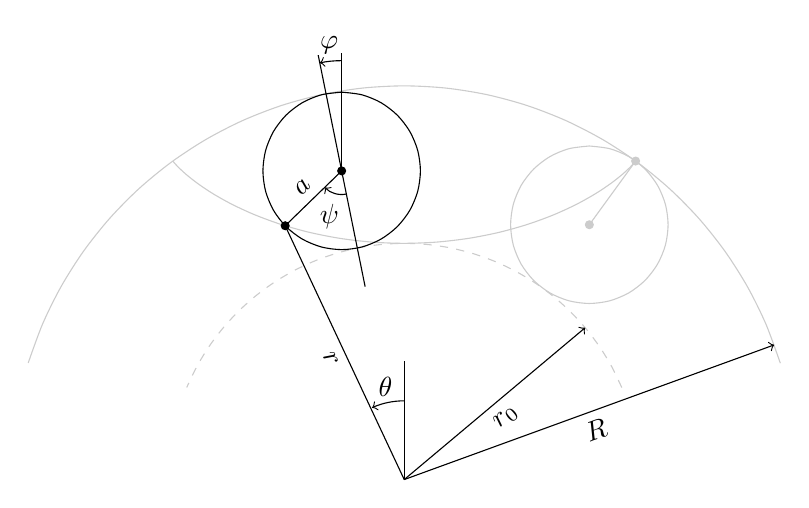
\begin{tikzpicture}
\pgfmathsetmacro{\R}{5.0}
\pgfmathsetmacro{\a}{1.0}
\pgfmathsetmacro{\Ra}{4.0}   % R-a
\pgfmathsetmacro{\aR}{0.2}   % a/R
\pgfmathsetmacro{\rnull}{3.0}   % R-2a
\pgfmathsetmacro{\cangle}{1.0}   % current angle (psi)

% outer circle
\draw[domain=0.3:3.141-0.3, smooth, variable=\t, color=black!20!white]
plot ({\R*cos(\t r)},{\R*sin(\t r))});

% inner circle
\draw[domain=0.4:3.141-0.4, smooth, variable=\t, color=black!20!white, dashed]
plot ({\rnull*cos(\t r)},{\rnull*sin(\t r))});

% hypocycloid
\draw[domain=-3.141:3.141, smooth, variable=\t, color=black!20!white]
plot ({-\Ra*sin(\aR*\t r) - \a*sin(-\aR*\t r + \t r)},{\Ra*cos(\aR*\t r) - \a*cos(-\aR*\t r + \t r )});

% initial state, circle and radius
\draw[domain=-3.141:3.141, smooth, variable=\t, color=black!20!white]
plot ({\Ra*sin(\aR*pi r) - \a*sin(\t r)},{\Ra*cos(\aR*pi r) - \a*cos(\t r)});
\draw[color=black!20!white, fill=black!20!white] ({\Ra*sin(\aR*pi r)},{\Ra*cos(\aR*pi r)}) circle[radius=0.05] -- ({\R*sin(\aR*pi r)},{\R*cos(\aR*pi r)}) circle[radius=0.05];

% current state, circle and radius
\draw[domain=-3.141:3.141, smooth, variable=\t]
plot ({\Ra*sin(-\aR*\cangle r) - \a*sin(\t r)}, {\Ra*cos(-\aR*\cangle r) - \a*cos(\t r)});

 \coordinate (A) at (0,0);   % center of large circle
 \coordinate (B) at ({-\Ra*sin(\aR*\cangle r)},{\Ra*cos(\aR*\cangle r)});   % center of small circle
 \coordinate (C) at ({-\Ra*sin(\aR*\cangle r) - \a*sin(-\aR*\cangle r + \cangle r)},{\Ra*cos(\aR*\cangle r) - \a*cos(-\aR*\cangle r + \cangle r)});   % point on hypocycloid
 \coordinate (Dp) at ({-1.5*sin(\aR*\cangle r)},{ 1.5*cos(\aR*\cangle r)});  % auxiliary point to denote angles
\coordinate (Dm) at ({ 1.5*sin(\aR*\cangle r)},{-1.5*cos(\aR*\cangle r)});  % auxiliary point to denote angles

 
\draw[fill=black] (B) circle[radius=0.05] -- node[above,sloped] {$a$} (C) circle[radius=0.05];

\draw (A) -- node[below,sloped] {$r$} (C);
\draw (A) -- (0, 1.5);
\draw (B) -- +(0, 1.5);
\draw (B) + (Dp) -- + (Dm);

\draw[->] (A) -- node[below,sloped] {$R$} (20:\R);
\draw[->] (A) -- node[below,sloped] {$r_0$} (40:\rnull);

\draw[->] (A)+(0,1) arc[start angle=90, end angle={90+2.1*deg(\aR*\cangle)}, radius=1];   % angle is MANUAL WORK
\draw (A)+({90+1*deg(\aR*\cangle)}:1.2) node {$\theta$};

\draw[->] (B)+(0,1.4) arc[start angle=90, end angle={90+deg(\aR*\cangle)}, radius=1.4];
\draw (B)+({90+deg(\aR*\cangle)/2}:1.6) node {$\varphi$};

\draw[->] (B)+({-90+deg(\aR*\cangle)}:0.3) arc[start angle={-90+deg(\aR*\cangle)}, end angle={-90-0.8*deg(\cangle)}, radius=0.3];
\draw (B)+(-105:0.6) node {$\psi$};

\end{tikzpicture}
 
